\section{Experiments and Results}

\subsection{Design Challenges}
\begin{enumroman}
  \item I spent a few hours debugging an issue with my hough transform,
    only to realize that I was writing \emph{into} my hough accumulator array
    when I do non-maximum suppression in \verb|myhoughLines.py| because I had not
    made a copy of the array.
    This was tough to identify, easy to fix --- and I later ran into another student with the same issue.
  \item Vectorizing code was pretty interesting,
    especially digging into \verb|numpy| documentation to figure out how to
    compose certain operations to get a desired result,
    and later realizing that there's yet another function that
    combines two or more of those operations.
    A huge lifesaver here was \verb|np.where|, which I didn't know existed
    before this assignment.
    I linked specific documentation links where relevant in the code.
\end{enumroman}

\subsection{Experiments}

I played around with some of the parameters to see how the results
are affected.

\begin{enumroman}
  \item \textbf{Gaussian kernel variance ($\sigma$):}
    Increasing the value of $\sigma$ improves the image detection up to a point,
    then flattens out the line once $\sigma$ goes beyond the optimal value.
    I found the best results with $\sigma = 2$ to work well for most of my images,
    although $\sigma = 3$ seemed to work better on one image.
  \item \textbf{Threshold:}
    Raising the threshold prunes erratic lines in the image,
    but if the threshold is too high, accurate lines are pruned too
    (see image).
    I found the best results with a threshold of $0.3$.

    \begin{figure}[h]
      % show images at 0.4 textwidth
      \centering
      % 0.03
      \begin{minipage}{0.4\textwidth}
        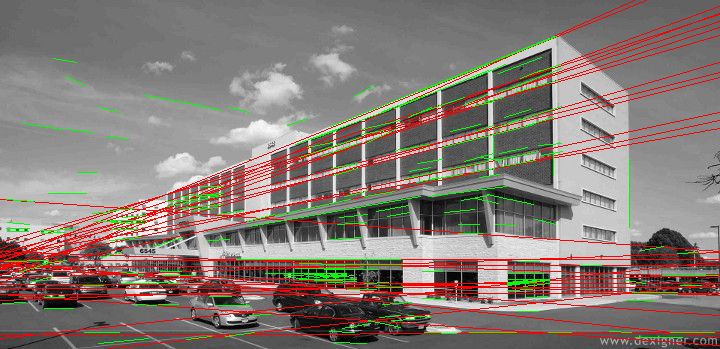
\includegraphics[width=\textwidth]{images/09-threshold-0.03.png}
        \caption{threshold = $0.03$}
        \label{fig:threshold-0.03}
      \end{minipage}
      \begin{minipage}{0.4\textwidth}
        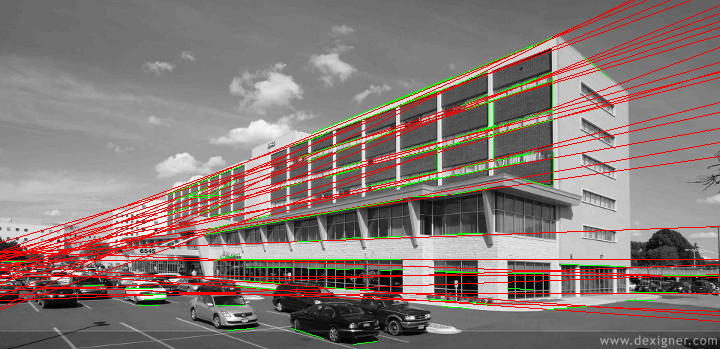
\includegraphics[width=\textwidth]{images/09-threshold-0.3.png}
        \caption{threshold = $0.3$}
        \label{fig:threshold-0.3}
      \end{minipage}
      % \hfill
      \begin{minipage}{0.4\textwidth}
        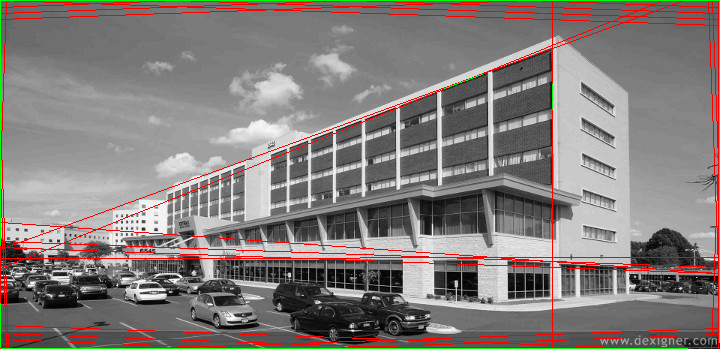
\includegraphics[width=\textwidth]{images/09-threshold-0.5.png}
        \caption{threshold = $0.5$}
        \label{fig:threshold-0.5}
      \end{minipage}
    \end{figure}
  \item \textbf{Theta Resolution:}
    Increasing the resolution of $\theta$ increases the accuracy
    of the lines found in the image, but it also increases the
    computation time. I found the best results with a resolution
    of $\frac{\pi}{180}$, but I settled on $\frac{\pi}{90}$
    because the reduction in accuracy is not too extreme,
    and it computes much faster.

  \item \textbf{Rho Resolution:}
    Increasing the $\rho$-resolution also increases the accuracy,
    but increases computation time.
    I thought $\rho$-resolution of $1$ was reasonable enough since
    the results looked good.

  \item \textbf{Number of Lines:}
    In general, finding more lines allows us to capture most of the lines
    in the image. However, it also eventually starts to make the image
    noisy as multiple lines that are close together get captured.

    The number of lines also needs to be tuned for each image,
    as a specific number of lines would work well in a specific image,
    then result in too much noise in another image.

    \begin{figure}[H]
      \centering
      \begin{minipage}{0.4\textwidth}
        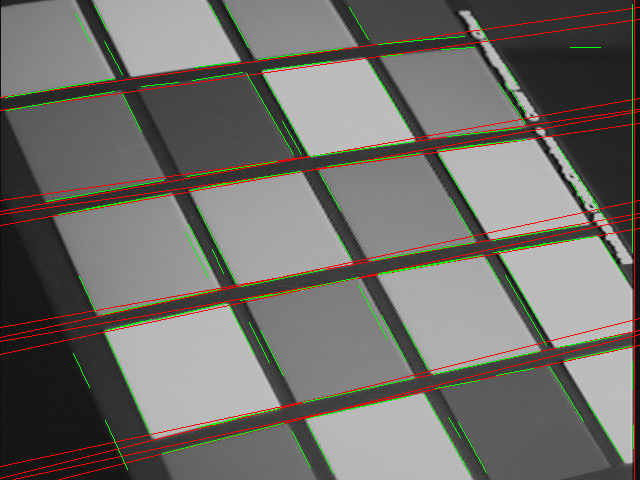
\includegraphics[width=\textwidth]{images/01-numlines-15.png}
        \caption{$15$ lines (misses all vertical lines)}
        \label{fig:lines-150}
      \end{minipage}
      \begin{minipage}{0.4\textwidth}
        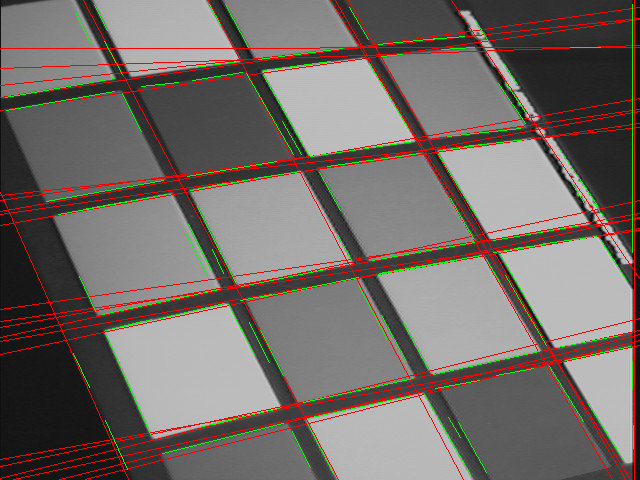
\includegraphics[width=\textwidth]{images/01-numlines-30.png}
        \caption{30 lines (a bit noisy but captures most)}
        \label{fig:lines-30}
      \end{minipage}
      \begin{minipage}{0.4\textwidth}
        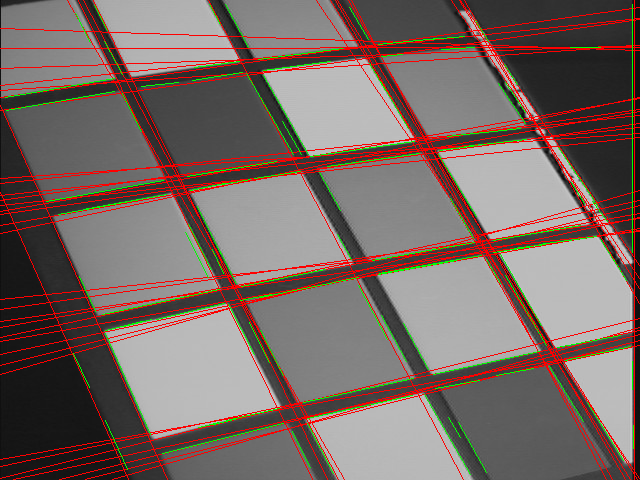
\includegraphics[width=\textwidth]{images/01-numlines-50.png}
        \caption{$50$ lines (too noisy)}
        \label{fig:lines-50}
      \end{minipage}
    \end{figure}
\end{enumroman}

\newpage
\subsection{Results}

These were the results I got for image 08.

\begin{figure}[H]
  \centering
  \begin{minipage}{0.4\textwidth}
    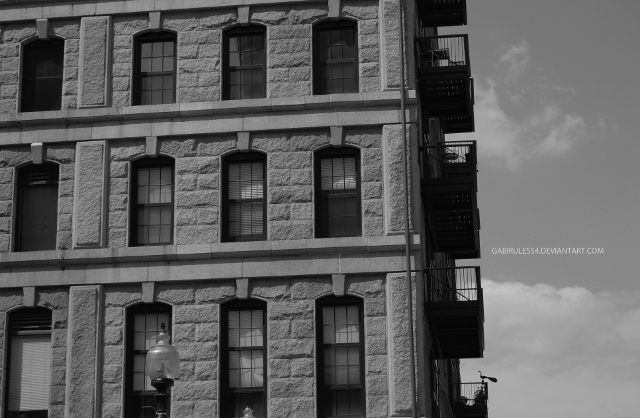
\includegraphics[width=\textwidth]{images/08-example-original.jpg}
    \caption{Original Image}
    \label{fig:08-original}
  \end{minipage}
  \begin{minipage}{0.4\textwidth}
    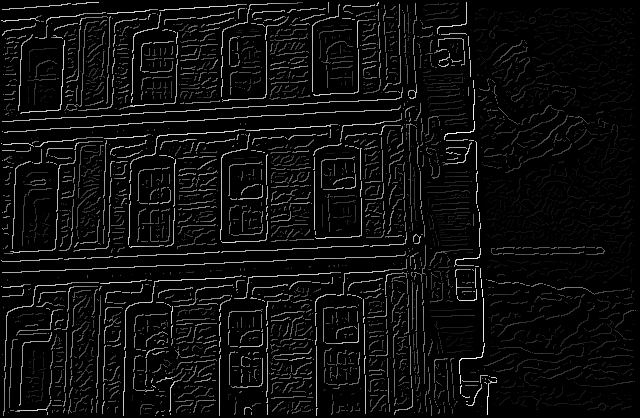
\includegraphics[width=\textwidth]{images/08-example-edges.png}
    \caption{Edges}
    \label{fig:08-edges}
  \end{minipage}
  \begin{minipage}{0.4\textwidth}
    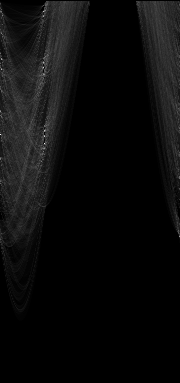
\includegraphics[width=\textwidth]{images/08-example-hough.png}
    \caption{Hough Transform}
    \label{fig:08-hough}
  \end{minipage}
  \begin{minipage}{0.4\textwidth}
    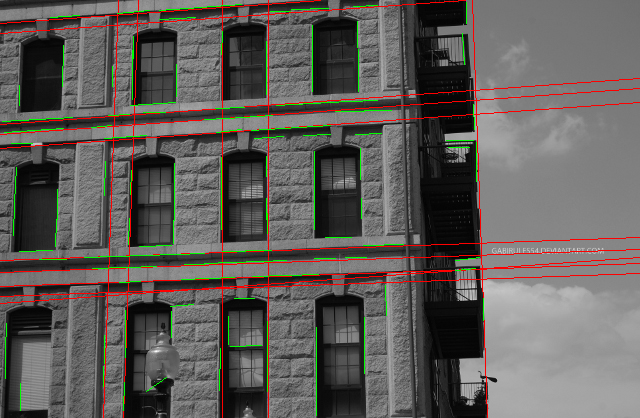
\includegraphics[width=\textwidth]{images/08-example-lines.png}
    \caption{Lines}
    \label{fig:08-lines}
  \end{minipage}
\end{figure}
